% 可自定义论文时间戳 \today
% \year=2021
% \month=5
% \day=20

\documentclass{sysuthesis} % 默认使用电子版(不填充空白页)。如果需要双面打印版,请注释掉本行并启用下一行
% \documentclass[print-both-sides]{sysuthesis} % 使用双面打印版(填充额外空白页以保证每一章开头都在奇数页)
\usepackage{sysucode}  % 在论文中使用代码

%%
% 论文相关信息
% 本文档中前缀"c-"代表中文版字段, 前缀"e-"代表英文版字段
% modifyer: 黄俊杰(huangjj27, 349373001dc@gmail.com)
% update date: 2017-04-13
%%

% 标题
% 论文题目应以简短、明确的词语恰当概括整个论文的核心内容,避免使用不常见的缩略词、缩写字。读者通过标题可大致了解毕业设计(论文)的内容、专业的特点和科学的范畴。中文题目一般不宜超过 24 个字,必要时可增加副标题。外文题目一般不宜超过 12 个实词

% 封面标题。由于技术所限,封面题目过长的划分交由用户您进行定夺
% 这也能让您的论文封面看起来更有美感
\covertitlefirst{中山大学}
\covertitlesecond{本科毕业论文(设计)} 
 
% Author:   Souler Ou
% 修改者:    欧一锋
% Date:     3/30/2018
% Mail:     ou@souler.cc
%如果英文标题过长可以使用此两项作为表三(答辩记录表)的标题。
\etitlefirst{\LaTeX \ Template}
\etitlesecond{for SYSU Graduation Thesis}

% 中文标题
\ctitle{中山大学本科毕业论文}
\etitle{ \LaTeX \ Template for SYSU Graduation Thesis}

% 作者详细信息
\author{王小明}
\cauthor{王\ 小\ 明}    % 封面作者
\eauthor{Wang Xiaoming}
\studentid{12350004}
\cschool{计算机学院}

\cmajor{计算机科学与技术}
\emajor{Computer Science and Technology}

% 指导老师
\cmentor{王大明 \ (教授)}
\ementor{Prof. 王大明}

     % 论文相关信息
%%
% 开题报告
% modifier: 黄俊杰(huangjj27, 349373001dc@gmail.com)
% update date: 2017-05-12

\proposal{
    测试开题报告意见
}

\proposalInstructions{
    测试指导老师意见
}

   % 开题报告内容
%%
% 摘要信息
% 本文档中前缀"c-"代表中文版字段, 前缀"e-"代表英文版字段
% 摘要内容应概括地反映出本论文的主要内容,主要说明本论文的研究目的、内容、方法、成果和结论。要突出本论文的创造性成果或新见解,不要与引言相 混淆。语言力求精练、准确,以 300—500 字为宜。
% 在摘要的下方另起一行,注明本文的关键词(3—5 个)。关键词是供检索用的主题词条,应采用能覆盖论文主要内容的通用技术词条(参照相应的技术术语 标准)。按词条的外延层次排列(外延大的排在前面)。摘要与关键词应在同一页。
% modifier: 黄俊杰(huangjj27, 349373001dc@gmail.com)
% update date: 2017-04-15
%%

\cabstract{

摘要应概括论文的主要信息,应具有独立性和自含性,即不阅读论文的全文,就能获得必要的信息。摘要内容一般应包括研究目的、内容、方法、成果和结论,要突出论文的创造性成果或新见解,不要与绪论相混淆。语言力求精练、准确,以300-500字为宜。关键词是供检索用的主题词条,应体现论文特色,具有语义性,在论文中有明确的出处,并应尽量采用《汉语主题词表》或各专业主题词表提供的规范词。关键词与摘要应在同一页,在摘要的下方另起一行注明,一般列3-5个,按词条的外延层次排列(外延大的排在前面)。

}
% 中文关键词(每个关键词之间用“,”分开,最后一个关键词不打标点符号。)
\ckeywords{本科毕业论文,\LaTeX\ 模板,中山大学}

\eabstract{
% 英文摘要及关键词内容应与中文摘要及关键词内容相同。中英文摘要及其关键词各置一页内。
The content of the English abstract is the same as the Chinese abstract, 250-400 content words are appropriate. Start another line below the abstract to indicate English keywords (Keywords 3-5).
}
% 英文文关键词(每个关键词之间用,分开, 最后一个关键词不打标点符号。)
\ekeywords{undergraduate thesis, \LaTeX\ template, Sun Yat-Sen University}

     % 摘要内容
%%
% 成绩评定记录表
% modifier: 黄俊杰(huangjj27, 349373001dc@gmail.com)
% update date: 2017-05-17

\gradingComment{
  某某同学针对什么问题研究了什么算法/实现了什么系统/针对这个系统做了什么测试,本文选题合理,实验结果表明技术路线……论文写作规范,引用文献充分,符合中山大学本科论文的规范,是篇优秀/良好/中等/合格的论文。
}
    % 成绩评定记录表评语
%%
% 四次进度报告相关信息

% Author:   Souler Ou
% 修改者:    欧一锋
% Date:     3/30/2018
% Mail:     ou@souler.cc

% 第一次进度报告
\firstsummary{
	\begin{adjustwidth}{2em}{2em}
		在这一阶段,XXX工作基本完成,主要在如下几个方面:
		\begin{enumerate}
			\item 完成了第一项。
			\item 完成了第二项
			\item 完成了第三项。
		\end{enumerate}
	\end{adjustwidth}
}
% 第2次进度报告
\secondsummary{
	\begin{adjustwidth}{2em}{2em}
		...
	\end{adjustwidth}
}
% 第3次进度报告
\thirdsummary{
	\begin{adjustwidth}{2em}{2em}
		...
	\end{adjustwidth}
}
% 第4次进度报告
\fourthsummary{
	\begin{adjustwidth}{2em}{2em}
		...
	\end{adjustwidth}
}
% 第1次老师评价
\firstcomment{
	\begin{adjustwidth}{2em}{2em}
		论文完成情况良好。
	\end{adjustwidth}
}
% 第2次老师评价
\secondcomment{
	\begin{adjustwidth}{2em}{2em}
		...
	\end{adjustwidth}
}
% 第3次老师评价
\thirdcomment{
	\begin{adjustwidth}{2em}{2em}
		...
	\end{adjustwidth}
}
% 第4次老师评价
\fourthcomment{
	\begin{adjustwidth}{2em}{2em}
		...
	\end{adjustwidth}
}
% 老师总评价
\finalcomment{
	\begin{adjustwidth}{2em}{2em}
		...
	\end{adjustwidth}
}   % 过程检查报告数据
\begin{document}
% 论文前置部分
\frontmatter
\pagenumbering{Roman}
\makeUndergraduateCover    % 封面
\makeUndergraduateTitlePage    % 扉页
% \makeProposal% 开题报告
% \makeProgressCheck  % 过程检查记录表
% \makeDefenseRecord  % 答辩情况等级表
\makedisclaim       % 学术诚信声明
\makeabstract       % 中英文摘要
\maketableofcontents        % 目录
\makelistoffiguretable

% 论文主体部分
\mainmatter
% 引言

% 正文
%%
% 引言或背景
% 引言是论文正文的开端,应包括毕业论文选题的背景、目的和意义;对国内外研究现状和相关领域中已有的研究成果的简要评述;介绍本项研究工作研究设想、研究方法或实验设计、理论依据或实验基础;涉及范围和预期结果等。要求言简意赅,注意不要与摘要雷同或成为摘要的注解。
% modifier: 黄俊杰(huangjj27, 349373001dc@gmail.com)
% update date: 2017-04-15
%%

\chapter{诸论}
%定义,过去的研究和现在的研究,意义,与图像分割的不同,going deeper
\label{cha:introduction}
\section{选题背景与意义}
\label{sec:background}
% What is the problem
% why is it interesting and important
% Why is it hards, why do naive approaches fails
% why hasn't it been solved before
% what are the key components of my approach and results, also include any specific limitations,do not repeat the abstract
%contribution
引言是论文正文的开端,应包括毕业论文选题的背景、目的和意义;对国内外研究现状和相关领域中已有的研究成果的简要评述;介绍本项研究工作研究设想、研究方法或实验设计、理论依据或实验基础;涉及范围和预期结果等。要求言简意赅,注意不要与摘要雷同或成为摘要的注解。

\section{国内外研究现状和相关工作}
\label{sec:related_work}
对国内外研究现状和相关领域中已有的研究成果的简要评述;
\section{本文的论文结构与章节安排}

\label{sec:arrangement}

本文共分为六章,各章节内容安排如下:

第一章诸论。简单说明了本文章的选题背景与意义。

第二章为本科生毕业论文写作与印制规范。本章节就学校的规范,逐点进行描述,并给出来了相关例子说明本模板在格式上的正确性。

第三章为本模板的使用说明。

第四章为可用的\LaTeX 的代码段方便大家进行编辑。

第五章是本文的最后一章,总结与展望。是对本文内容的整体性总结以及对未来工作的展望。


\newclearpage
\chapter{本科生毕业论文写作与印制规范}

\label{cha:sysu-thesis-contents-format-requirement}


% TODO 引用
该部分将学校规定中的毕业论文(设计)写作与印制规范复制了过来,并在其中展示相关例子表明格式的正确性。


\section{毕业论文的撰写内容与要求}

\subsection{封面}


纸质版封面由学校统一印发(电子版请参见文后示例)。封面内容包括论文题目、所在院系专业、学生姓名学号、指导教师(姓名及职称)等信息。论文题目应以简短、明确的词语恰当概括整个论文的核心内容,避免使用不常见的缩略词、缩写字。读者通过题目可大致了解毕业论文的内容、专业特点和学科范畴。论文题目一般不宜超过25个字,必要时可增加副标题。

\subsection{扉页}

扉页内容包括论文中英文题目、学生姓名、学号、院系、专业、指导教师(姓名及职称)等信息。格式详见文后示例。

\subsection{学术诚信声明}

内容及格式详见文后示例。

\subsection{摘要和关键词}

\begin{enumerate}
    \item \textbf{中文摘要和关键词} \\
          摘要应概括论文的主要信息,应具有独立性和自含性,即不阅读论文的全文,就能获得必要的信息。摘要内容一般应包括研究目的、内容、方法、成果和结论,要突出论文的创造性成果或新见解,不要与绪论相混淆。语言力求精练、准确,以300-500字为宜。关键词是供检索用的主题词条,应体现论文特色,具有语义性,在论文中有明确的出处,并应尽量采用《汉语主题词表》或各专业主题词表提供的规范词。关键词与摘要应在同一页,在摘要的下方另起一行注明,一般列3-5个,按词条的外延层次排列(外延大的排在前面)。
    \item \textbf{英文摘要和关键词} \\
          英文摘要及关键词内容应与中文摘要及关键词内容相同。中英文摘要及其关键词各置一页内。
\end{enumerate}

\subsection{目录}

目录是论文的提纲,也是论文各章节组成部分的小标题。要求标题层次清晰,目录中的标题要与正文中的标题一致。


\subsection{正文}

正文是毕业论文的主体和核心部分,不同学科专业和不同的选题可以有不同的写作方式。正文一般包括以下几个方面:

\begin{enumerate}
    \item \textbf{诸论} \\
          绪论应包括毕业论文选题的背景、目的和意义;对国内外研究现状和相关领域中已有的研究成果的简要评述;介绍本项研究工作研究设想、研究方法或实验设计、理论依据或实验基础;涉及范围和预期结果等。要求言简意赅,注意不要与摘要雷同或成为摘要的注解。
    \item \textbf{主体} \\
          论文主体是毕业论文的主要部分,必须言之成理,论据可靠,严格遵循本学科国际通行的学术规范。在写作上要注意结构合理、层次分明、重点突出,章节标题、公式图表符号必须规范统一。论文主体的内容根据不同学科有不同的特点,一般应包括以下几个方面:
          \begin{enumerate}
              \item 毕业论文总体方案或选题的论证;
              \item 毕业论文各部分的设计实现,包括实验数据的获取、数据可行性及有效性的处理与分析、各部分的设计计算等;
              \item 对研究内容及成果的客观阐述,包括理论依据、创新见解、创造性成果及其改进与实际应用价值等;
              \item 论文主体的所有数据必须真实可靠,凡引用他人观点、方案、资料、数据等,无论曾否发表,无论来源于纸质或电子版材料,均应详加注释。自然科学论文应推理正确、结论清晰;人文和社会学科的论文应把握论点正确、论证充分、论据可靠,恰当运用系统分析和比较研究的方法进行模型或方案设计,注重实证研究和案例分析,根据分析结果提出建议和改进措施等。
          \end{enumerate}
    \item \textbf{结论} \\
          结论是毕业论文的总结,是整篇论文的归宿,应精炼、准确、完整。结论应着重阐述自己的创造性成果及其在本研究领域中的意义和作用,还可进一步提出需要讨论的问题和建议。
\end{enumerate}

\subsection{参考文献}

参考文献是毕业论文不可缺少的组成部分,它反映毕业论文的取材来源、材料的广博和可靠程度,也是作者对他人知识成果的承认和尊重。凡有引用他人的著作、论文等,均应列于参考文献中。

\subsection{相关的科研成果目录}

本科期间发表的与毕业论文相关的论文或被鉴定的技术成果、发明专利等,应在成果目录中列出。此项不是必需项,空缺时可以省略。

\subsection{附录}

对于一些不宜放在正文中的重要支撑材料,可编入毕业论文的附录中,包括某些重要的原始数据、详细数学推导、程序全文及其说明、复杂的图表、设计图纸等一系列需要补充提供的说明材料。如果毕业论文中引用的实例、数据资料,实验结果等符号较多时,为了节约篇幅,便于读者查阅,可以编写一个符号说明,注明符号代表的意义。附录的篇幅不宜太多,一般不超过正文。此项不是必需项,空缺时可以省略。

\subsection{致谢}

致谢应以简短的文字对课题研究与论文撰写过程中曾直接给予帮助的人员(例如指导教师、答疑教师及其他人员)表达自己的谢意,这不仅是一种礼貌,也是对他人劳动的尊重,是治学者应当遵循的学术规范。内容限一页。


\section{毕业论文的撰写格式要求}


\subsection{文字和字数}


除外国语言文学类专业外,其他专业的毕业论文须采用简化汉语文字撰写。论文正文部分一般不少于8000 字,各专业可根据需要确定具体的字数要求,并报教务部备案。

\subsection{字体和字号}

标题一般用黑体,内容一般用宋体,数字和英文字母一般用Times New Roman,具体如\autoref{tab:font-spec}。

\begin{table}[]
    \caption{字体使用规范}
    \begin{tabular}{|c|c|}
        \hline
        论文题目               & 黑体二号居中                                  \\ \hline
        中文摘要标题           & 黑体三号居中                                  \\ \hline
        中文摘要内容           & 宋体小四号                                    \\ \hline
        中文关键词             & 宋体小四号(标题``关键词''加粗)              \\ \hline
        英文摘要标题           & Times New Roman加粗三号全部大写               \\ \hline
        英文摘要内容           & Times New Roman小四号                         \\ \hline
        英文关键词             & Times New Roman小四号(标题``Keywords''加粗) \\ \hline
        目录标题               & 黑体三号居中                                  \\ \hline
        目录内容               & 宋体小四号                                    \\ \hline
        正文各章标题           & 黑体三号居中                                  \\ \hline
        正文各节一级标题       & 黑体四号左对齐                                \\ \hline
        正文各节二级及以下标题 & 宋体小四号加粗左对齐空两格                    \\ \hline
        正文内容               & 宋体小四号                                    \\ \hline
        参考文献标题           & 黑体三号居中                                  \\ \hline
        参考文献内容           & 宋体五号                                      \\ \hline
        致谢、附录标题         & 黑体三号居中                                  \\ \hline
        致谢、附录内容         & 宋体小四号                                    \\ \hline
        页眉与页脚             & 宋体五号居中                                  \\ \hline
        图题、表题             & 宋体五号                                      \\ \hline
        脚注、尾注             & 宋体小五号                                    \\ \hline
    \end{tabular}
    \label{tab:font-spec}
\end{table}


字体样例可见如下(以居中形式展现): \\



\begin{center}
    {\heiti\zihao{2}黑体二号居中} \\

    {\heiti\zihao{3}黑体三号居中} \\

    {\heiti\zihao{4}黑体四号居中} \\

    {\songti\zihao{4}宋体四号居中} \\

    {\songti\zihao{-4}宋体小四号居中} \\

    {\songti\zihao{5}宋体五号居中} \\

    {\songti\zihao{-5}宋体小五号居中} \\

    {\zihao{3} Times New Roman : Three} 三号居中 \\

    {\zihao{-4} Times New Roman : Small Four} 小四号居中 \\

\end{center}


\subsection{页面设置}

纸张大小:A4。

页边距:上边距25 mm,下边距20 mm,左右边距均为30 mm。

行距:1.5倍行距,章和节标题段前段后各空0.5行。

\subsection{页码}

页面底端居中,从摘要开始至绪论之前以大写罗马数字(
\uppercase\expandafter{\romannumeral1} ,
\uppercase\expandafter{\romannumeral2} ,
\uppercase\expandafter{\romannumeral3} ,
…)单独编连续码,绪论开始至论文结尾,以阿拉伯数字(1,2,3…)编连续码。

\subsection{关键词}


摘要正文下方另起一行顶格打印``关键词''款项,后加冒号,多个关键词以逗号分隔。

\subsection{目录}

目录应另起一页,包括论文中的各级标题,按照``一……''、``(一)……''或``1……''、``1.1……''格式编写。

\subsection{各级标题}

正文各部分的标题应简明扼要,不使用标点符号。论文内文各大部分的标题用``一、二……(或1、2……)'',次级标题为``(一)、(二)……(或1.1、2.1……)'',三级标题用``1、2……(或1.1.1、2.1.1……)'',四级标题用``(1)、(2)……(或1.1.1.1、2.1.1.1……)'',不再使用五级以下标题。两类标题不要混编。

\subsection{名词术语}

\begin{enumerate}
    \item 科学技术名词术语尽量采用全国自然科学名词审定委员会公布的规范词或国家标准、部标准中规定的名称,尚未统一规定或叫法有争议的名词术语,可采用惯用的名称。
    \item 特定含义的名词术语或新名词、以及使用外文缩写代替某一名词术语时,首次出现时应在括号内注明其含义,如:经济合作与发展组织(Organisation for Economic Co-operation and Development, OECD)。
    \item 外国人名一般采用英文原名,可不译成中文,英文人名按姓前名后的原则书写,如:CRAY P,不可将外国人姓名中的名部分漏写,例如:不能只写CRAY, 应写成CRAY P。一般很熟知的外国人名(如牛顿、爱因斯坦、达尔文、马克思等)可按通常标准译法写译名。
\end{enumerate}

\subsection{物理量名称、符号与计量单位}

\begin{enumerate}
    \item 论文中某一物理量的名称和符号应统一,应采用国务院发布的《中华人民共和国法定计量单位》、国际公认或各行业领域惯用的计量单位。单位名称和符号的书写方式,应采用国际通用符号。
    \item 在不涉及具体数据表达时允许使用中文计量单位如``千克''。
    \item 表达时刻应采用中文计量单位,如``下午3点10分'',不能写成``3h10min'',在表格中可以用``3:10PM''表示。
    \item 物理量符号、物理量常量、变量符号用斜体,计量单位符号均用正体。
\end{enumerate}

\subsection{数字}

\begin{enumerate}
    \item 无特别约定情况下,一般均采用阿拉伯数字表示。
    \item 年份一律使用4位数字表示。
          % \item 统计符号的格式:一般除$\mu$、$\alpha$、$\beta$、$\lambda$、$\varepsilon$ 以及$V$等符号外,其余统计符号一律以斜体字呈现,如$ANCOVA$,$ANOVA$,$MANOVA$,$N$,$nl$,$M$,$SD$,$F$,$p$,$r$等。
    \item 统计符号的格式:一般除μ、α、β、λ、ε以及V等符号外,其余统计符号一律以斜体字呈现,如\textit{ANCOVA},\textit{ANOVA},\textit{MANOVA},\textit{N},\textit{nl},\textit{M},\textit{SD},\textit{F},\textit{p},\textit{r}等。
\end{enumerate}


\subsection{公式}

\begin{enumerate}
    \item 公式应另起一行写在稿纸中央。一行写不完的长公式,最好在等号处转行,如做不到这一点,可在运算符号(如``+''、``-''号)处转行,等号或运算符号应在转行后的行首。
    \item 公式的编号用圆括号括起,放在公式右边行末,在公式和编号之间不加虚线。公式可按全文统编序号,也可按章编独立序号,如(49)、(4.11)、(4-11)等。采用哪一种序号应和图序、表序编法一致。不应出现某章里的公式编序号,有的则不编序号。子公式可不编序号,需要引用时可加编a、b、c……,重复引用的公式不得另编新序号。公式序号必须连续,不得重复或跳缺。
    \item 文中引用某一公式时,可写成``由式(序号)''。
\end{enumerate}

\ \\

这是一个例子:

\begin{equation}
    \label{eq:example-formulas}
    ax^2 +bx+c = 0
\end{equation}


如\autoref{eq:example-formulas}所示,为了求解该一元二次方程,我们可以推导得到该方程的求根公式。因此,由\autoref{eq:example-formulas2}即可求解该方程的两个根。

\begin{equation}
    \label{eq:example-formulas2}
    \begin{split}
        x_1 = & \frac{-b+\sqrt{b^2-4ac}}{2a} \\
        & \\
        x_2 = & \frac{-b-\sqrt{b^2-4ac}}{2a}
    \end{split}
\end{equation}

\subsection{表格}

\begin{enumerate}
    \item 表格必须与论文叙述有直接联系,不得出现与论文叙述脱节的表格。表格中的内容在技术上不得与正文矛盾。
    \item 每个表格都应有自己的标题和序号。标题应写在表格上方正中,不加标点,序号写在标题左方。
    \item 全文的表格可以统一编序,也可以逐章单独编序。采用哪一种方式应和插图、公式的编序方式统一。表序必须连续,不得跳缺。
    \item 表格允许下页接写,接写时标题省略,表头应重复书写,并在右上方写``续表××''。多项大表可以分割成块,多页书写,接口处必须注明``接下页''、``接上页''、``接第×页''字样。
    \item 表格应放在离正文首次出现处最近的地方,不应超前和过分拖后。
\end{enumerate}


例子可见\autoref{tab:table-example}。

\begin{table}[!htbp]
    \centering
    \caption{表格例子}
    \label{tab:table-example}
    \begin{tabular}{|l|l|}
        \hline
        \multicolumn{1}{|c|}{这是表格第一行第一列} & 这是表格第一行第二列 \\ \hline
        这是表格第二行第一列                       & 这是表格第二行第二列 \\ \hline
    \end{tabular}
\end{table}

\subsection{图}


\begin{enumerate}
    \item 插图应与文字内容相符,技术内容正确。所有制图应符合国家标准和专业标准。对无规定符号的图形应采用该行业的常用画法。
    \item 每幅插图应有标题和序号,全文的插图可以统一编序,也可以逐章单独编序,采取哪一种方式应和表格、公式的编序方式统一。图序必须连续,不重复,不跳缺。
    \item 由若干分图组成的插图,分图用a、b、c……标序。分图的图名以及图中各种代号的意义,以图注形式写在图题下方,先写分图名,另起行写代号的意义。
    \item 图与图标题、图序号为一个整体,不得拆开排版为两页。当页空白不够排版该图整体时,可将其后文字部分提前,将图移至次页最前面。
    \item 对坐标轴必须进行文字标示,有数字标注的坐标图必须注明坐标单位。
\end{enumerate}

例子可见\autoref{fig:example-figure}。

\begin{figure}[!htbp]
    \centering
    \includegraphics[width=3cm]{example-image-a}
    \caption{图片例子}
    \label{fig:example-figure}
\end{figure}

\subsection{注释}

毕业论文(设计)中有个别名词或情况需要解释时,可加注说明。注释采用脚注或尾注,应根据注释的先后顺序编排序号。注释序号以``①、②''等数字形式标示在正文中被注释词条的右上角,脚注或尾注内容中的序号应与被注释词条序号保持一致。

脚注例子可见这里\footnote{这是一个脚注}。

\subsection{参考文献}

参考文献的序号左顶格,并用数字加方括号表示,如``[1]''。每一条参考文献著录均以``.''结束。各类参考文献的具体编排格式请参照国家标准《信息与文献 参考文献著录规则》(GB/T 7714-2015)。

参考文献例子可见这里\cite{sysu-thesis}。


\subsection{附录}

论文附录依次用大写字母``附录A、附录B、附录C……''表示,附录内的分级序号可采用``附A1、附A1.1、附A1.1.1''等表示,图、表、公式均依此类推为``图A1、表A1、式A1''等。

% TODO:增加引用例子。
\newclearpage
\chapter{研究方法}
\label{cha:method}

\newclearpage
\chapter{简单的使用例子}
\label{cha:usage-example}

本部分将会根据毕设论文的写作需要,放置相关的例子和代码段供大家参考,方便大家的论文写作,如果更多有用的Latex使用例子也会欢迎提出PR,贡献更多的例子。

\section{图像的插入}

\subsection{镶嵌在文中的图像}
\begin{wrapfigure}{r}{0.5\linewidth}
    \centering
    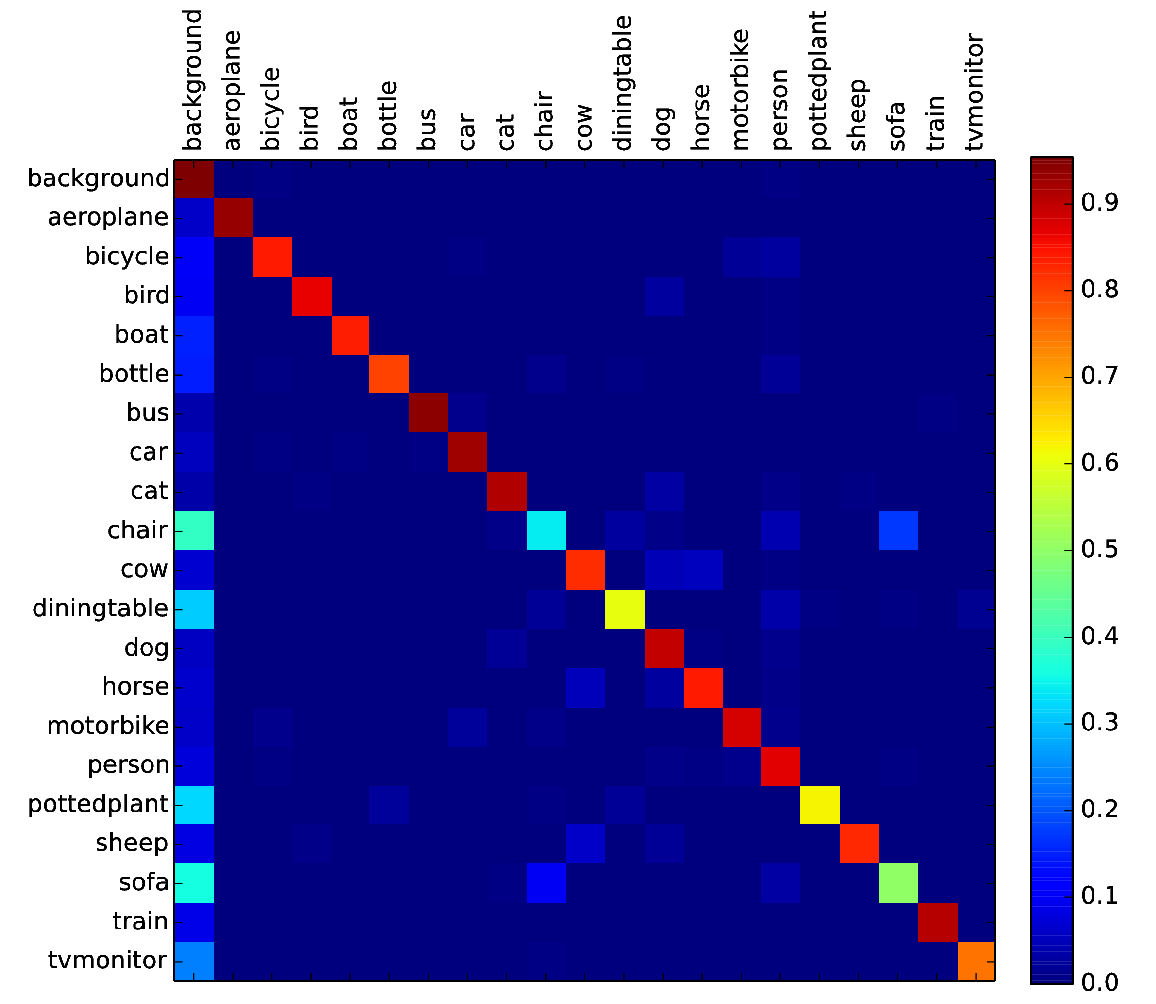
\includegraphics[width=0.5\textwidth]{image/chap04/confusion.pdf}
    \caption{镶嵌在文中的图像}
    \label{fig:image-embedding-text}
\end{wrapfigure}
论文主体是毕业论文的主要部分,必须言之成理,论据可靠,严格遵循本学科国际通行的学术规范。在写作上要注意结构合理、层次分明、重点突出,章节标题、公式图表符号必须规范统一。论文主体的内容根据不同学科有不同的特点,一般应包括以下几个方面: (1)毕业论文(设计)总体方案或选题的论证; (2)毕业论文(设计)各部分的设计实现,包括实验数据的获取、数据可行性及有效性的处理与分析、各部分的设计计算等; (3)对研究内容及成果的客观阐述,包括理论依据、创新见解、创造性成果及其改进与实际应用价值等; (4)论文主体的所有数据必须真实可靠,凡引用他人观点、方案、资料、数据等,无论曾否发表,无论是纸质或电子版,均应详加注释。自然科学论文应推理正确、结论清晰;人文和社会学科的论文应把握论点正确、论证充分、论据可靠,恰当运用系统分析和比较研究的方法进行模型或方案设计,注重实证研究和案例分析,根据分析结果提出建议和改进措施等。
论文主体是毕业论文的主要部分,必须言之成理,论据可靠,严格遵循本学科国际通行的学术规范。在写作上要注意结构合理、层次分明、重点突出,章节标题、公式图表符号必须规范统一。论文主体的内容根据不同学科有不同的特点,一般应包括以下几个方面: (1)毕业论文(设计)总体方案或选题的论证; (2)毕业论文(设计)各部分的设计实现,包括实验数据的获取、数据可行性及有效性的处理与分析、各部分的设计计算等; (3)对研究内容及成果的客观阐述,包括理论依据、创新见解、创造性成果及其改进与实际应用价值等; (4)论文主体的所有数据必须真实可靠,凡引用他人观点、方案、资料、数据等,无论曾否发表,无论是纸质或电子版,均应详加注释。自然科学论文应推理正确、结论清晰;人文和社会学科的论文应把握论点正确、论证充分、论据可靠,恰当运用系统分析和比较研究的方法进行模型或方案设计,注重实证研究和案例分析,根据分析结果提出建议和改进措施等。



\subsection{单张图像的插入}

\begin{figure}[h]
    \centering
    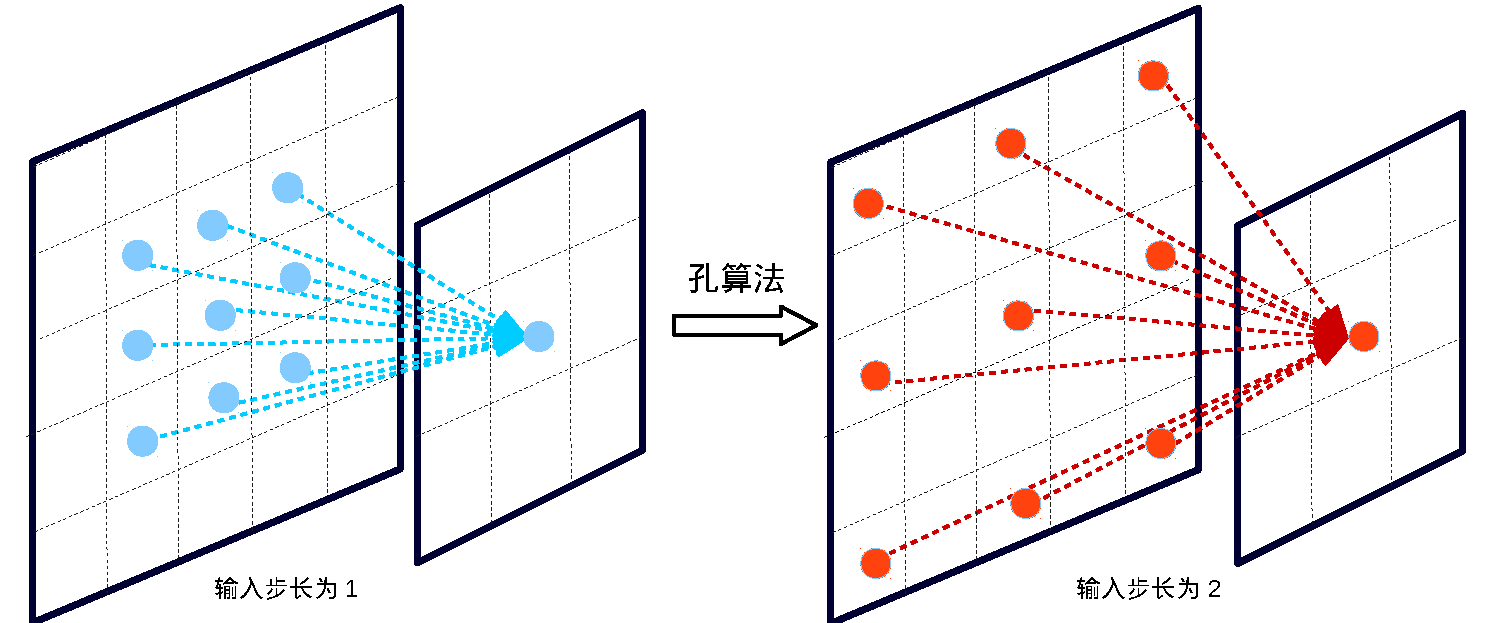
\includegraphics[width=0.5\textwidth]{image/chap04/illustration/hole.pdf}
    \caption{单张图像}
     \label{fig:hole}
\end{figure}


\subsection{多张图像的并排插入}


\begin{figure}[h!]%文中的Grid-LSTM模型做的语义图像分割的例子
    \centering
    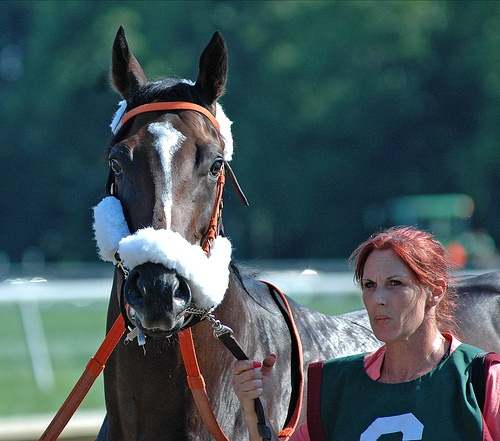
\includegraphics[width=.2\textwidth,height=.15\textwidth]{image/chap04/example/2007_000799.jpg}
    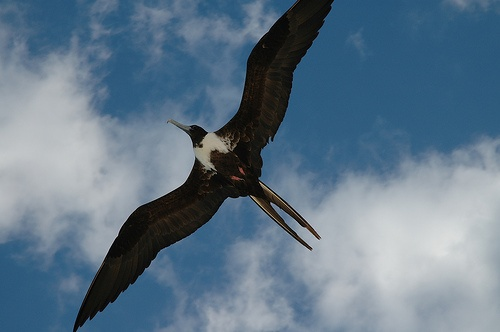
\includegraphics[width=.2\textwidth,height=.15\textwidth]{image/chap04/example/2007_002094.jpg}
    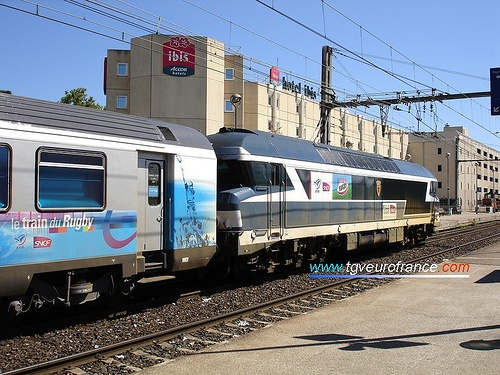
\includegraphics[width=.2\textwidth,height=.15\textwidth]{image/chap04/example/2007_004483.jpg}
    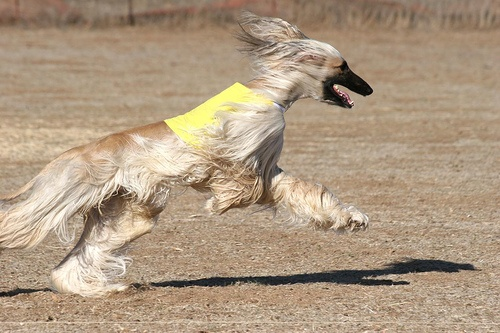
\includegraphics[width=.2\textwidth,height=.15\textwidth]{image/chap04/example/2007_003194.jpg}
    \\
    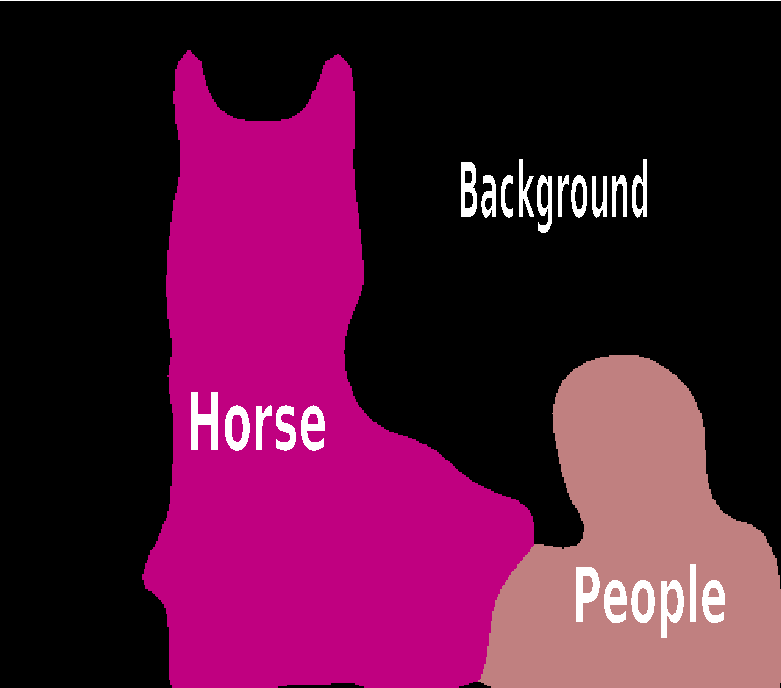
\includegraphics[width=.2\textwidth,height=.15\textwidth]{image/chap04/example/2007_000799.pdf}
    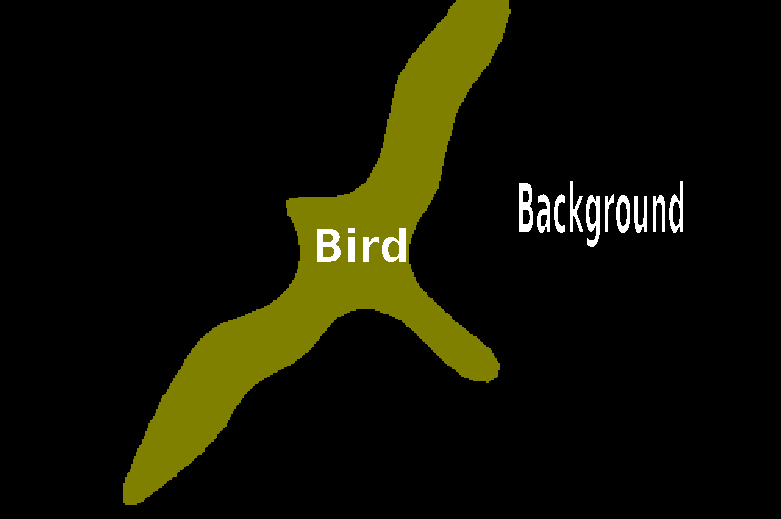
\includegraphics[width=.2\textwidth,height=.15\textwidth]{image/chap04/example/2007_002094.pdf}
    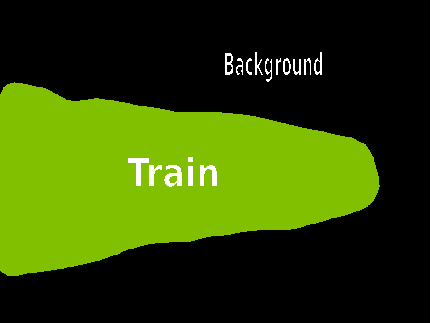
\includegraphics[width=.2\textwidth,height=.15\textwidth]{image/chap04/example/2007_004483.pdf}
    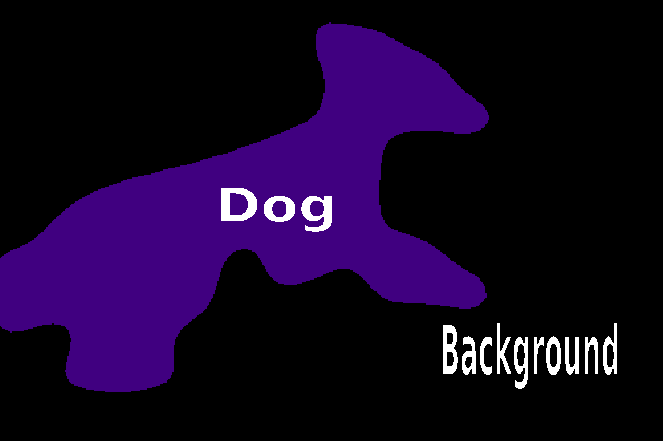
\includegraphics[width=.2\textwidth,height=.15\textwidth]{image/chap04/example/2007_003194.pdf}
    \caption{并排的多张图像}
    \label{fig:multi-image-example1}
\end{figure}


\begin{figure}[h]
    \centering
        \makebox[0.11\textwidth]{\scriptsize 图像}
        \enspace
        \makebox[0.11\textwidth]{\scriptsize 真值}
        \enspace
        \makebox[0.11\textwidth]{\scriptsize CNN+5LSTM\textbf{1}}
        \enspace\thinspace
        \makebox[0.11\textwidth]{\scriptsize CNN+5LSTM\textbf{2}}
        \enspace\thinspace
        \makebox[0.11\textwidth]{\scriptsize CNN+5LSTM\textbf{3}}
        \enspace\thinspace
        \makebox[0.11\textwidth]{\scriptsize CNN+5LSTM\textbf{4}}
        \enspace\thinspace
        \makebox[0.11\textwidth]{\scriptsize CNN+5LSTM\textbf{5}}\\
        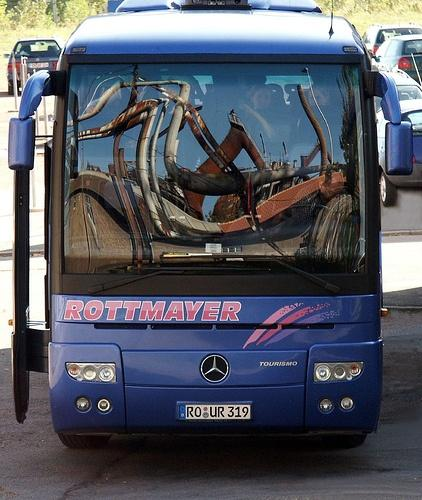
\includegraphics[width=0.11\textwidth]{image/chap04/improvement/2007_000663.jpg}
        \enspace\thinspace %\hfill
        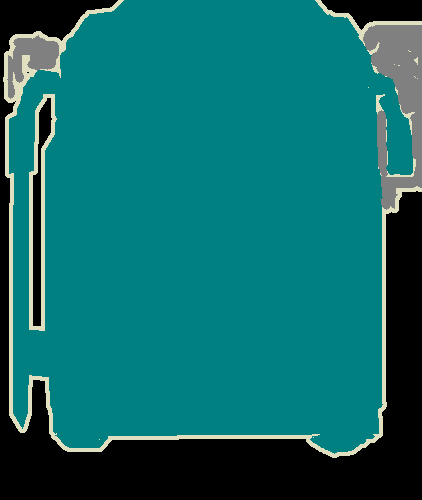
\includegraphics[width=0.11\textwidth]{image/chap04/improvement/2007_000663.png}
        \enspace\thinspace
        
\includegraphics[width=0.11\textwidth]{image/chap04/improvement/2007_000663_1.png}
        \enspace\thinspace
        
\includegraphics[width=0.11\textwidth]{image/chap04/improvement/2007_000663_2.png}
        \enspace\thinspace
        
\includegraphics[width=0.11\textwidth]{image/chap04/improvement/2007_000663_3.png}
        \enspace\thinspace
        
\includegraphics[width=0.11\textwidth]{image/chap04/improvement/2007_000663_4.png}
        \enspace\thinspace
        
\includegraphics[width=0.11\textwidth]{image/chap04/improvement/2007_000663_5.png}
        \enspace\thinspace
        \caption{并排的多张图像加各自的注解}
        \label{fig:improvement}
\end{figure}
    

\subsection{两列图像的插入}

\begin{figure}[h!] % image examples & compare
    \begin{subfigure}{0.55\textwidth}
        \makebox[0.18\textwidth]{\scriptsize Grid-5LSTM}
        \makebox[0.18\textwidth]{\scriptsize FCN-8s\cite{long2015fully}}
        \makebox[0.18\textwidth]{\scriptsize SDS\cite{hariharan2014simultaneous}}
        \makebox[0.18\textwidth]{\scriptsize 真值}
        \makebox[0.18\textwidth]{\scriptsize 图像} \\
        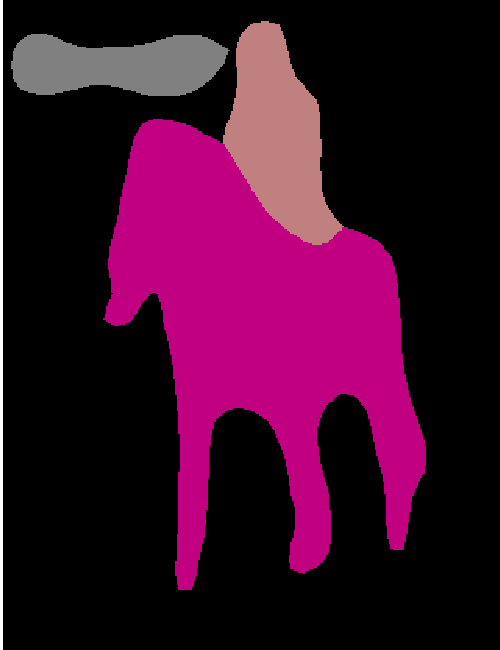
\includegraphics[width=0.18\textwidth]{image/chap04/result/compare/my_horse.pdf}
        
\includegraphics[width=0.18\textwidth]{image/chap04/result/compare/fcn_horse.png}
        
\includegraphics[width=0.18\textwidth]{image/chap04/result/compare/sds_horse.png}
        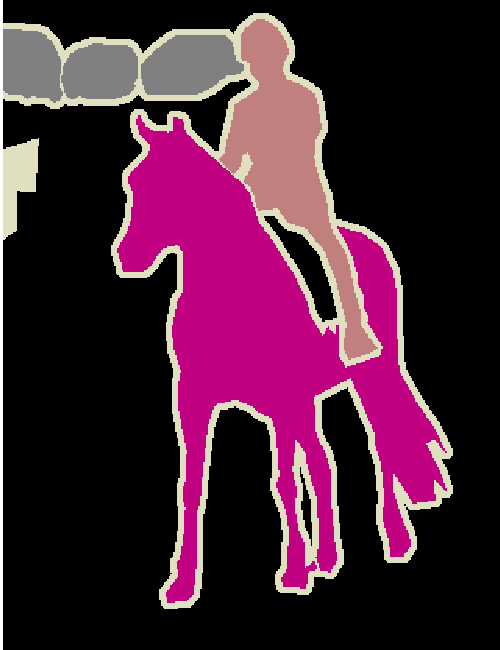
\includegraphics[width=0.18\textwidth]{image/chap04/result/compare/gt_horse.pdf}
        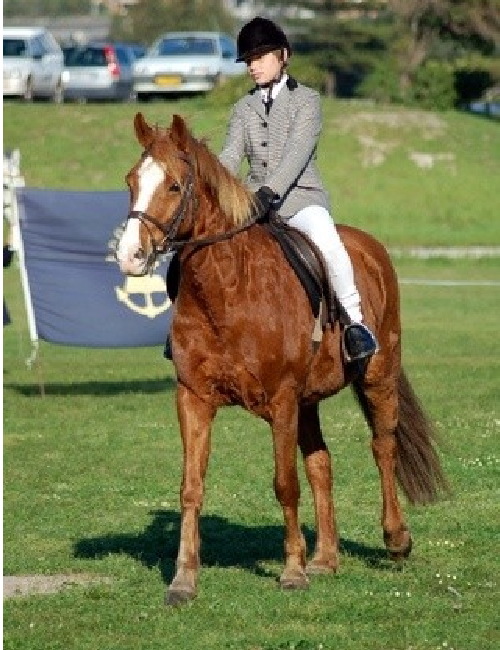
\includegraphics[width=0.18\textwidth]{image/chap04/result/compare/im_horse.pdf}
        \\
        
\includegraphics[width=0.18\textwidth]{image/chap04/result/compare/my_motor.png}
        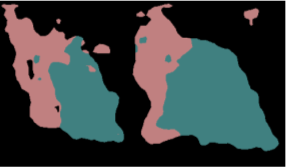
\includegraphics[width=0.18\textwidth]{image/chap04/result/compare/fcn_motor.png}
        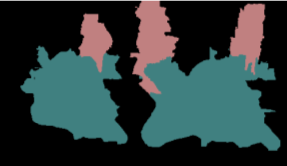
\includegraphics[width=0.18\textwidth]{image/chap04/result/compare/sds_motor.png}
        
\includegraphics[width=0.18\textwidth]{image/chap04/result/compare/2007_005173.png}
        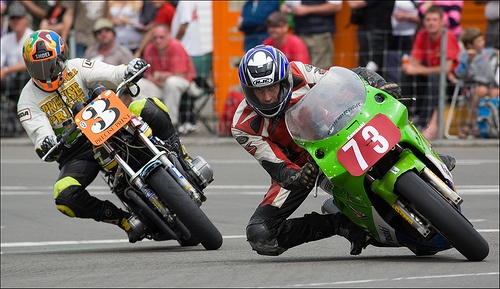
\includegraphics[width=0.18\textwidth]{image/chap04/result/compare/2007_005173.jpg}
        \\
        
\includegraphics[width=0.18\textwidth]{image/chap04/result/compare/my_sheep.pdf}
        
\includegraphics[width=0.18\textwidth]{image/chap04/result/compare/fcn_sheep.png}
        
\includegraphics[width=0.18\textwidth]{image/chap04/result/compare/sds_sheep.png}
        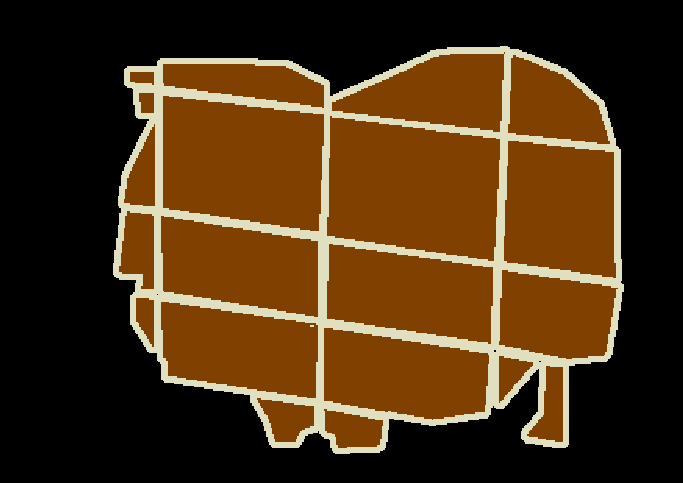
\includegraphics[width=0.18\textwidth]{image/chap04/result/compare/gt_sheep.pdf}
        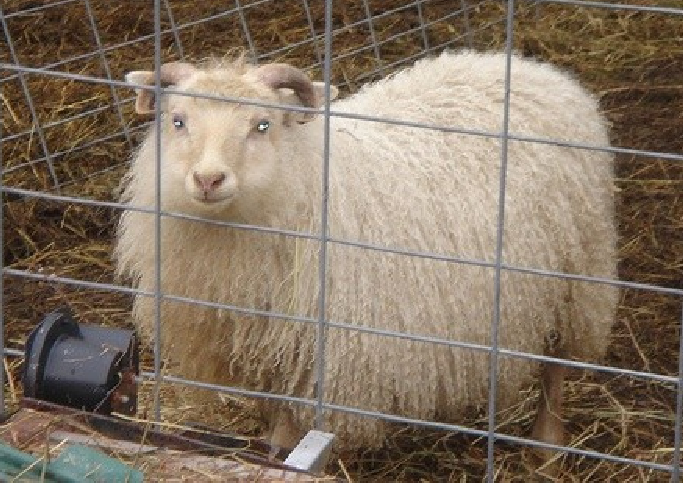
\includegraphics[width=0.18\textwidth]{image/chap04/result/compare/im_sheep.pdf}
        \\
        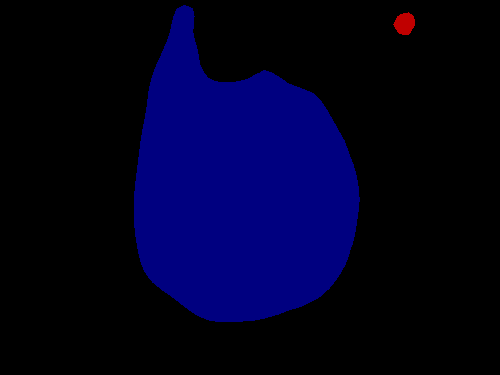
\includegraphics[width=0.18\textwidth]{image/chap04/result/compare/my_boat.png}
        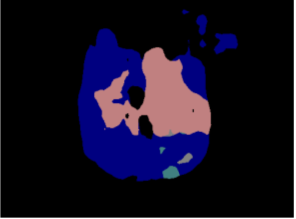
\includegraphics[width=0.18\textwidth]{image/chap04/result/compare/fcn_boat.png}
        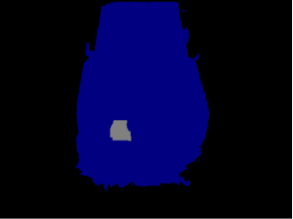
\includegraphics[width=0.18\textwidth]{image/chap04/result/compare/sds_boat.png}
        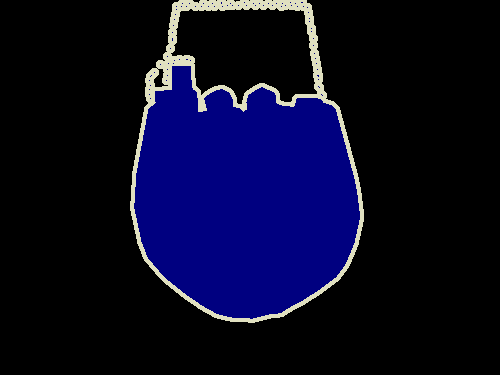
\includegraphics[width=0.18\textwidth]{image/chap04/result/compare/2007_004241.png}
        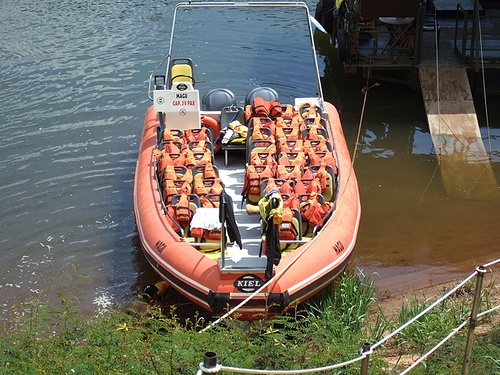
\includegraphics[width=0.18\textwidth]{image/chap04/result/compare/2007_004241.jpg}
        \caption{左边的图像}
        \label{fig:compare1}
    \end{subfigure}
    \begin{subfigure}{0.4\textwidth}
        \centering
%		\makebox[0.3\textwidth]{} \\
%		\makebox[0.3\textwidth]{} \\
        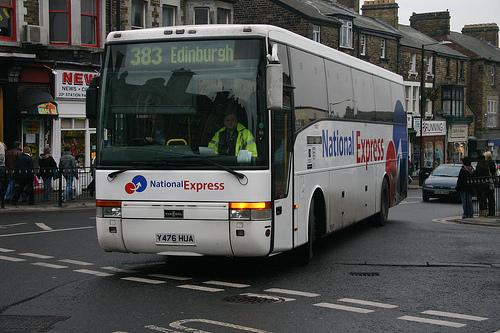
\includegraphics[width=0.25\textwidth]{image/chap04/result/compare/2010_005284.jpg}
        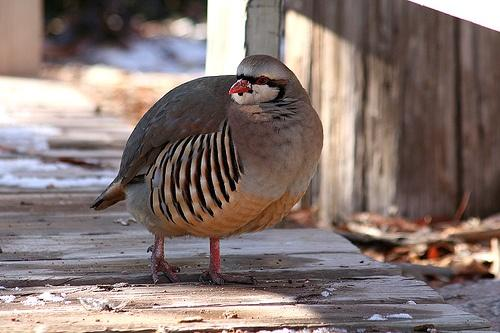
\includegraphics[width=0.25\textwidth]{image/chap04/result/compare/2007_003349.jpg}
        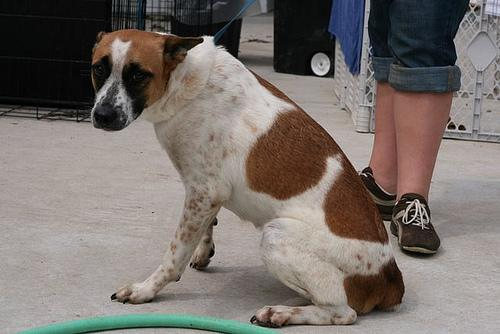
\includegraphics[width=0.25\textwidth]{image/chap04/result/compare/2009_004507.jpg} 
        \\
        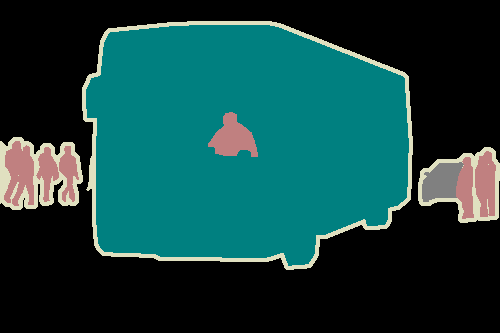
\includegraphics[width=0.25\textwidth]{image/chap04/result/compare/2010_005284.png}
        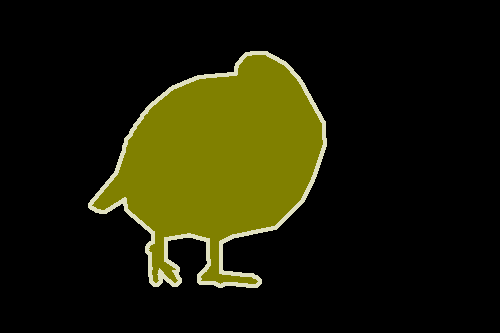
\includegraphics[width=0.25\textwidth]{image/chap04/result/compare/2007_003349.png}
        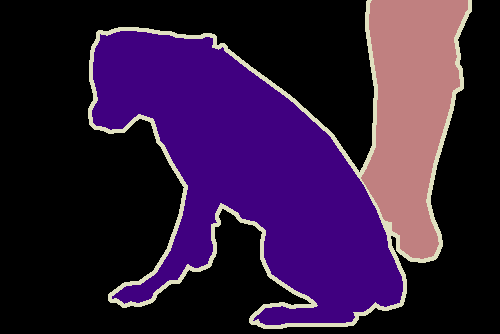
\includegraphics[width=0.25\textwidth]{image/chap04/result/compare/2009_004507.png} \\
        
\includegraphics[width=0.25\textwidth]{image/chap04/result/compare/zoom_bus.png}
        
\includegraphics[width=0.25\textwidth]{image/chap04/result/compare/zoom_bird.png}
        
\includegraphics[width=0.25\textwidth]{image/chap04/result/compare/zoom_dog.png} \\
        
\includegraphics[width=0.25\textwidth]{image/chap04/result/compare/deeplab_bus.png}
        
\includegraphics[width=0.25\textwidth]{image/chap04/result/compare/deeplab_bird.png}
        
\includegraphics[width=0.25\textwidth]{image/chap04/result/compare/deeplab_dog.png} \\
        \includegraphics[width=0.25\textwidth]{image/chap04/result/compare/my_bus.png}
        \includegraphics[width=0.25\textwidth]{image/chap04/result/compare/my_bird.png}
        \includegraphics[width=0.25\textwidth]{image/chap04/result/compare/my_dog.png} 
        \caption{右边的图像}
        \label{fig:compare2}
    \end{subfigure}
    \caption{复杂的两列对象的插入}
    \label{fig:complex}
\end{figure}


\clearpage

\section{表格的插入}

\begin{table}[h] %voc table result
    \centering
        \caption{典型的实验对比表格}
        \begin{tabular}{*{4}{c}}
            \toprule
             Method & Pixel Acc. & Mean Acc. & Mean Iu.\\
            \midrule
            Liu等人\cite{liu2011sift}  & 76.7 & - & -\\
        Tighe等人\cite{tighe2013finding}  & 78.6 & 39.2 & -\\
            FCN-16s\cite{long2015fully} & 85.2 & \textbf{51.7} & 39.5\\
            Deeplab-LargeFOV\cite{chen14semantic} & 85.6 & 51.2 & 39.7\\
            \midrule
            Grid-LSTM5 & \textbf{86.2} & 51.0 & \textbf{41.2}\\
            \bottomrule
        \end{tabular}
        \label{tab:siftflow}
\end{table}

\begin{table}[h] %voc table result
    \centering
        \caption{复杂一些的表格}
        \resizebox{\textwidth}{!}{
        \begin{tabular}{c|*{20}{c}|c}
            \toprule
            Method & aero & bike & bird & boat & bottle & bus & car & cat & chair & cow & table & dog & horse & mbike & person & plant & shep & sofa & train & tv & mIoU.\\
            \midrule
            CNN				   & 72.6 & 29.6 & 70.2 & 53.1 & 65.1 & 81.0 & 74.3 & 79.8 & 25.0 & 64.8 & 47.8 & 69.5 & 66.2 & 65.2 & 74.2 & 42.1 & 69.6 & 38.8 & 74.4 & 58.6 & 62.5\\
            CNN+\textbf{1}LSTM & 71.5 & 30.6 & 70.5 & 53.8 & 64.9 & 82.4 & 77.1 & 79.5 & 25.1 & 65.8 & 47.8 & 71.5 & 64.6 & 67.0 & 74.0 & 43.9 & 69.6 & 38.6 & 74.9 & 59.4 & 63.0\\
            CNN+\textbf{2}LSTM & 76.1 & 32.6 & 72.1 & 57.0 & 65.3 & 83.6 & 75.4 & 81.7 & 24.7 & 69.3 & 47.5 & 72.3 & 68.9 & 69.5 & 74.7 & 41.5 & 69.8 & 38.3 & 77.8 & 62.1 & 64.3 \\
            CNN+\textbf{3}LSTM & 77.7 & 32.3 & 72.6 & 60.0 & 68.3 & 85.5 & 78.5 & 82.3 & 25.3 & 71.1 & 49.7 & 71.5 & 69.7 & 70.8 & 75.9 & 47.9 & 71.2 & 38.9 & 80.2 & 61.7 & 65.8 \\
            CNN+\textbf{4}LSTM & 79.1 & \textbf{33.7} & \textbf{73.6} & \textbf{62.0} & \textbf{70.4} & 85.5 & \textbf{80.9} & 83.7 & \textbf{24.1} & 70.7 & 45.7 & 73.7 & 69.6 & 72.1 & 75.6 & 47.2 & \textbf{76.0} & 37.3 & 80.5 & 62.2 & 66.4 \\
            CNN+\textbf{5}LSTM & \textbf{79.9} & 33.6 & \textbf{73.6} & 61.7 & 68.0 & \textbf{88.5} & \textbf{80.9} & \textbf{84.0} & 23.6 & \textbf{71.3} & \textbf{49.7} & \textbf{73.1} & \textbf{71.3} & \textbf{72.9} & \textbf{76.4} & \textbf{48.9} & 75.1 & \textbf{38.1} & \textbf{84.5} & \textbf{63.8} & \textbf{67.2} \\
            \midrule
            CNN+\textbf{5}LSTM$^\dag$ & 84.8 & 36.4 & 82.0 & 69.4 & 73.0 & 87.2 & 81.8 & 86.1 & 34.5 & 82.4 & 53.1 & 81.5 & 77.4 & 79.0 & 81.3 & 54.8 & 81.1 & 47.0 & 84.3 & 67.3 & 72.3 \\
            \bottomrule
        \end{tabular}}
        \label{tab:vocval}
    \end{table}
    

\section{公式}
\label{sec:formula}
没有编号的公式
\begin{align*}
\begin{split}
    \label{eq:feedforward}
    \mybold{z}^{(l)} & = \mybold{W}^{(l)}\mybold{a}^{(l-1)} + \mybold{b}^{(l)} \\
    \mybold{a}^{(l)} & = f(\mybold{z}^{(l)})
\end{split}
\end{align*}
公式中含有中文
\begin{align}
    \begin{split}
    \mbox{像素准确率} &= \sum_{i=1}^{n_{cl}}n_{ii} / \sum_{i=1}^{n_{cl}}t_i \\
        \mbox{平均像素准确率} &= \frac{1}{n_{cl}} \sum_{i=1}^{n_{cl}}(n_{ii}/ t_i) \\
    \mbox{Mean IU} &= \frac{1}{n_{cl}} \sum_{i=1}^{n_{cl}}\frac{n_{ii}}{t_i + \sum_j^{n_{cl}} n_{ji} - n_{ii}}
    \end{split}
\end{align}
公式中含有矩阵
\begin{equation}
    \textbf{H} = \begin{bmatrix}
        I*\mybold{x}_i \\ \textbf{h}
    \end{bmatrix}
\end{equation}
每行后面都有编号的公式
\begin{align}
    \frac{\partial}{\partial W_{ij}^{(l)}} J(\mybold{W},\mybold{b};\mybold{x},y) &= \frac{\partial J(\mybold{W},\mybold{b};\mybold{x},y)}{\partial z_i^{(l+1)}}\cdot \frac{\partial z_i^{(l+1)}}{\partial W_{ij}^{(l)}} = \delta_i^{(l+1)}a_j^{(l)} \\
    \frac{\partial}{\partial b_i^{(l)}} J(\mybold{W},\mybold{b};\mybold{x},y) &= \frac{\partial J(\mybold{W},\mybold{b};\mybold{x},y)}{\partial z_i^{(l+1)}}\cdot \frac{\partial z_i^{(l+1)}}{\partial b_i^{(l)}} = \delta_i^{(l+1)}
\end{align}

\section{算法流程图}
\label{sec:algorithm}
\begin{algorithm}[h]
\KwIn{$m$个训练样本}
\lFor{$l=1$ \emph{\KwTo} $n_l$}{
初始化:$\Delta \mybold{W}^{(l)}=0$,$\Delta \mybold{b}^{(l)}=0$}
\ForEach{训练样本}{
    \lFor{$l=1$ \emph{\KwTo} $n_l-1$}{
    前向传播:$\mybold{z}^{(l+1)}=\mybold{W}^la^l+\mybold{b}^l$,$\mybold{a}^{(l+1)}=f(\mybold{z}^{(l+1)})$}
    输出误差计算:$\delta^{(n_l)} = \frac{\partial}{\partial \mybold{z}^{(n_l)}} J(\mybold{W},\mybold{b};\mybold{x},y)$\;
    \lFor{$l=n_l-1$ \emph{\KwTo} $1$}{
    后向传播:$\delta^{(l)} = \bigl((\mybold{W}^{(l)})^T \delta^{(l+1)}\bigr)f'(\mybold{z}^{(l)})$}
    \ForAll{层l}{
        计算梯度:$\nabla_{\mybold{W}^{(l)}}J(\mybold{W},\mybold{b};\mybold{x},y)=\delta^{(l+1)}(\mybold{a}^{(l)})^T$ \\
        \hspace{60pt}$\nabla_{\mybold{b}^{(l)}}J(\mybold{W},\mybold{b};\mybold{x},y)=\delta^{(l+1)}$\;
        累加梯度:$\Delta \mybold{W}^{(l)} \leftarrow \Delta \mybold{W}^{(l)} + \nabla_{\mybold{W}^{(l)}}J(\mybold{W},\mybold{b};\mybold{x},y)$; \\
        \hspace{60pt}$\Delta \mybold{b}^{(l)} \leftarrow \Delta \mybold{b}^{(l)} + \nabla_{\mybold{b}^{(l)}}J(\mybold{W},\mybold{b};\mybold{x},y)$\;
    }
}
\ForAll{层$l$}{
    更新权重:$\mybold{W}^{(l)} \leftarrow \mybold{W}^{(l)} - \alpha \biggl[\frac 1m \Delta \mybold{W}^{(l)}\biggr]$ \\
    \hspace{60pt} $\mybold{b}^{(l)} \leftarrow \mybold{b}^{(l)} - \alpha \biggl[\frac 1m \Delta \mybold{b}^{(l)}\biggr]$
}
\caption{梯度下降算法}
\label{algo:sgd}
\end{algorithm}

\section{例子、定理与证明}

\begin{eg}
  这是一个例子, 用以验证特殊环境的字体成功更改为楷体.
\end{eg}

\begin{theorem}[定理例子]
    \label{the:example-theorem}
    这是一个定理。
\end{theorem}

\begin{corollary}[推论例子]
    \label{the:example-corollary}
    这是一个推论。
\end{corollary}

\begin{lemma}[引理例子]
    \label{the:example-lemma}
    这是一个引理。
\end{lemma}

这里我们先给出\autoref{the:example-theorem-sysu-thesis}

\begin{theorem}[中山大学毕业论文模板定理]
\label{the:example-theorem-sysu-thesis}
中山大学 \LaTeX 毕业论文模板\cite{sysu-thesis}可以用于写各种证明。
\end{theorem}

下面我们对\autoref{the:example-theorem-sysu-thesis}进行证明:


\begin{proof}

下面我们开始证明:

由本定理的证明可见,我可以引用\autoref{the:example-theorem}和引理\ref{the:example-corollary}以及推论\ref{the:example-lemma}来证明我这个 \LaTeX 可以用来写各种证明。 \\

\autoref{the:example-theorem-sysu-thesis}得证。
\end{proof}

\section{代码}

本模版支持在论文中插入代码片段,或直接从源码文件进行插入。
例如,在论文中插入代码片段的效果为:
\begin{python}
def func():
    print("hello world")
    with open('./output.txt', 'w') as f:
        L = f.readlines()

if __name__ == "__main__":
    # this is a comment line
    func()
\end{python}
也可在行内插入代码片段,例如:Python中重载加法运算符的函数为\pyinline{__add__},类的标识符为\pyinline{class}。
此外,还可直接插入代码文件,例如插入\texttt{./code/demo.cpp}的效果为:
\lstinputlisting[style=sysucpp]{code/demo.cpp}


\section{其他的一些用法}
\label{sec:font}
\subsection{子章节编号}
\label{sec:font:subsection}
\subsubsection{更小的章节}
\label{sec:font:subsection:subsub}
更小的章节编号也是支持的。

可以如此引用章节:

\begin{itemize}
    \item \autoref{cha:usage-example}
    \item  \autoref{sec:font}
    \item  \autoref{sec:font:subsection}
    \item  \autoref{sec:font:subsection:subsub}
\end{itemize}


\subsection{列表的使用}
\label{sec:font:list}

这是一个无序列表
\begin{itemize}
    \item 引用文献\cite{long2015fully}
    \item 字体{\color{red}{变红}},\textbf{粗体},\textit{斜体},\underline{下划线}。
\end{itemize}

这是一个有序列表
\begin{enumerate}
    \item 索引前面的\autoref{sec:formula}、图像\ref{fig:complex}、表格\ref{tab:siftflow}
    \item 加脚注\footnote{测{\zihao{-5}试一下}脚注和URL \url{http://cs231n.github.io/transfer-learning/}}
\end{enumerate}



\newclearpage
\chapter{研究方法}
\label{cha:method}

\newclearpage

% 结语

% 附录部分
\backmatter
% 参考文献. 因不需要纳入章节目录, 故放入附录部分
% 实际上参考文献是属于论文主体部分
\makereferences

% 附录
{
    \appendix
    \chapter{补充更多细节}

\section{补充图}

\subsection{补充图}

这是附录内容,应该用宋体小四号字体。

\begin{figure}[h!]
	\centering
	\makebox[0.16\textwidth]{\scriptsize 图像}
	\makebox[0.16\textwidth]{\scriptsize 真值}
	\makebox[0.16\textwidth]{\scriptsize Grid-5LSTM1}
	\makebox[0.16\textwidth]{\scriptsize Grid-5LSTM3}
	\makebox[0.16\textwidth]{\scriptsize Grid-5LSTM5} \\
	\includegraphics[width=0.16\textwidth]{image/appendix1/2007_000042.jpg}
	\includegraphics[width=0.16\textwidth]{image/appendix1/2007_000042.png}
	\includegraphics[width=0.16\textwidth]{image/appendix1/1/2007_000042.png}
	\includegraphics[width=0.16\textwidth]{image/appendix1/3/2007_000042.png}
	\includegraphics[width=0.16\textwidth]{image/appendix1/5/2007_000042.png} \\

	\includegraphics[width=0.16\textwidth]{image/appendix1/2011_003256.jpg}
	\includegraphics[width=0.16\textwidth]{image/appendix1/2011_003256.png}
	\includegraphics[width=0.16\textwidth]{image/appendix1/1/2011_003256.png}
	\includegraphics[width=0.16\textwidth]{image/appendix1/3/2011_003256.png}
	\includegraphics[width=0.16\textwidth]{image/appendix1/5/2011_003256.png} \\
	\includegraphics[width=0.16\textwidth]{image/appendix1/2011_001159.jpg}
	\includegraphics[width=0.16\textwidth]{image/appendix1/2011_001159.png}
	\includegraphics[width=0.16\textwidth]{image/appendix1/1/2011_001159.png}
	\includegraphics[width=0.16\textwidth]{image/appendix1/3/2011_001159.png}
	\includegraphics[width=0.16\textwidth]{image/appendix1/5/2011_001159.png} \\
	\includegraphics[width=0.16\textwidth]{image/appendix1/2011_000813.jpg}
	\includegraphics[width=0.16\textwidth]{image/appendix1/2011_000813.png}
	\includegraphics[width=0.16\textwidth]{image/appendix1/1/2011_000813.png}
	\includegraphics[width=0.16\textwidth]{image/appendix1/3/2011_000813.png}
	\includegraphics[width=0.16\textwidth]{image/appendix1/5/2011_000813.png} \\
	\includegraphics[width=0.16\textwidth]{image/appendix1/2011_003145.jpg}
	\includegraphics[width=0.16\textwidth]{image/appendix1/2011_003145.png}
	\includegraphics[width=0.16\textwidth]{image/appendix1/1/2011_003145.png}
	\includegraphics[width=0.16\textwidth]{image/appendix1/3/2011_003145.png}
	\includegraphics[width=0.16\textwidth]{image/appendix1/5/2011_003145.png} \\
	\includegraphics[width=0.16\textwidth]{image/appendix1/2009_004579.jpg}
	\includegraphics[width=0.16\textwidth]{image/appendix1/2009_004579.png}
	\includegraphics[width=0.16\textwidth]{image/appendix1/1/2009_004579.png}
	\includegraphics[width=0.16\textwidth]{image/appendix1/3/2009_004579.png}
	\includegraphics[width=0.16\textwidth]{image/appendix1/5/2009_004579.png} \\
	\color[rgb]{0.9,0.9,0.9}\bfseries
	\begin{tabular}{*{7}{>{\centering\arraybackslash}p{0.10\textwidth}}}
		\hline
		\cellcolor[rgb]{0,0,0}  背景                 & \cellcolor[rgb]{0.5020,0,0} 飞机         & \cellcolor[rgb]{0,0.5020,0} 自行车 & \cellcolor[rgb]{0.5020,0.5020,0} 鸟 & \cellcolor[rgb]{0,0,0.5020} 船        & \cellcolor[rgb]{0.5020,0,0.5020} 瓶子 & \cellcolor[rgb]{0,0.5020,0.5020} 大巴
		\\
		\hline
		\cellcolor[rgb]{0.5020,0.5020,0.5020} 汽车   & \cellcolor[rgb]{0.2510,0,0} 猫           & \cellcolor[rgb]{0.7529,0,0} 椅子   & \cellcolor[rgb]{0.2510,0.5020,0} 牛 & \cellcolor[rgb]{0.7529,0.5020,0} 桌子 & \cellcolor[rgb]{0.2510,0,0.5020} 狗   & \cellcolor[rgb]{0.7529,0,0.5020} 马   \\
		\hline
		\cellcolor[rgb]{0.2510,0.5020,0.5020} 摩托车 & \cellcolor[rgb]{0.7529,0.5020,0.5020} 人 & \cellcolor[rgb]{0,0.2510,0} 盆栽   & \cellcolor[rgb]{0.5020,0.2510,0} 羊 & \cellcolor[rgb]{0,0.7529,0} 沙发      & \cellcolor[rgb]{0.5020,0.7529,0} 火车 & \cellcolor[rgb]{0,0.2510,0.5020} 电视 \\
		\hline
	\end{tabular}

	\caption{一个配有彩色表格的插图}
\end{figure}

\endinput

    \newclearpage
}

%%
% 致谢
% 谢辞应以简短的文字对课题研究与论文撰写过程中曾直接给予帮助的人员(例如指导教师、答疑教师及其他人员)表示对自己的谢意,这不仅是一种礼貌,也是对他人劳动的尊重,是治学者应当遵循的学术规范。内容限一页。
% modifier: 黄俊杰
% update date: 2017-04-15
%%

\chapter{致谢}

	四年时间转眼即逝,青涩而美好的本科生活快告一段落了。回首这段时间,我不仅学习到了很多知识和技能,而且提高了分析和解决问题的能力与养成了一定的科学素养。虽然走过了一些弯路,但更加坚定我后来选择学术研究的道路,实在是获益良多。这一切与老师的教诲和同学们的帮助是分不开的,在此对他们表达诚挚的谢意。

	首先要感谢的是我的指导老师林倞教授。我作为一名本科生,缺少学术研究经验,不能很好地弄清所研究问题的重点、难点和热点,也很难分析自己的工作所能够达到的层次。林老师对整个研究领域有很好的理解,以其渊博的知识和敏锐的洞察力给了我非常有帮助的方向性指导。他严谨的治学态度与辛勤的工作方式也是我学习的榜样,在此向林老师致以崇高的敬意和衷心的感谢。

	最后我要感谢我的家人,正是他们的无私的奉献和支持,我才有了不断拼搏的信息的勇气,才能取得现在的成果。

\vskip 108pt
\begin{flushright}
	陈冠英\makebox[1cm]{} \\
\today
\end{flushright}

    % 致谢
\newclearpage

% \makeGrade      % 成绩评定记录表
\end{document}
